\chapter{Анализ проблематики \dots}
\label{chapter1}

Это обзорно-аналитическая глава, в которой требуется отразить:

\begin{itemize}
	\item результат изучения различных существующих методов решения задач в рамках проблематики УИРа/диплома (иногда даже в смежных областях), это обзорный аспект, который пишется, в основном, на основе имеющейся литературы или/и программного обеспечения;
	\item сравнение (с какой-либо определенной целью) этих методов и средств.
\end{itemize}

Приведенные ниже названия пунктов являются очень примерными, их состав и структура сильно зависят от специфики конкретной работы.




%Большие отсупы --- это хорошо. Облегчает чтение длинных <<простыней>> текста
\section{Общий анализ проблематики \dots}

\begin{annotation}
В случае РСПЗ, так оформляется аннотация к разделу. Такая же аннотация, только более общая, должна быть для главы. После аннотации может следовать рабочая или финальная версия текста соответствующего раздела. В случае ПЗ, таких аннотаций быть не должно.
\end{annotation}

\dots

Результаты анализа полезно оформлять в виде таблиц (см. табл. \ref{tbl:cmp-1}).

\begin{table}%
\caption{Результаты сравнения нескольких программных систем}\label{tbl:cmp-1}
\centering
\begin{tabular}{|l|l|c|c|c|c|}

\hline

\textnumero & Название системы & Показатель 1 & Показатель 2 & Показатель 3 & Показатель 4 \\

\hline

\end{tabular}
\end{table}


\section{Анализ особенностей \dots}

Сначала приведем пример более сложной таблицы (см. табл. \ref{tbl:cmp-adv} и 
\ref{tbl:cmp-2}).

\begin{table}%
\caption{Таблица с длинным, многострочным названием, чтобы показать, как форматируется такой заголовок}
\label{tbl:cmp-adv}
\centering
\begin{tabular}{|l|l|c|c|c|c|}

\hline

\textnumero & Название системы & Показатель 1 & Показатель 2 & Показатель 3 & Показатель 4 \\

\hline

\end{tabular}
\label{tbl:cmp-2}
\end{table}


А теперь, продемонстрируем, как должна выглядеть иллюстрация (см. рис. \ref{pic:lambda-cube}).

\begin{figure}[t]%
\begin{center}
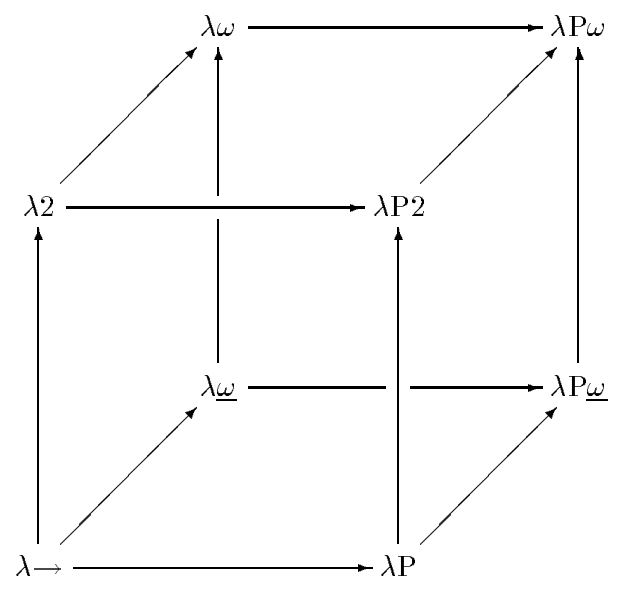
\includegraphics[width=.5\columnwidth]{./img/lambda-cube.png}%
\end{center}
\caption{Ламбда-куб Барендрегта}%
\label{pic:lambda-cube}%
\end{figure}

А теперь, продемонстрируем, как должна выглядеть иллюстрация с длинной подрисуночной подписью (см. рис. \ref{pic:lambda-cube-long-caption}).

\begin{figure}[t]%
	\begin{center}
		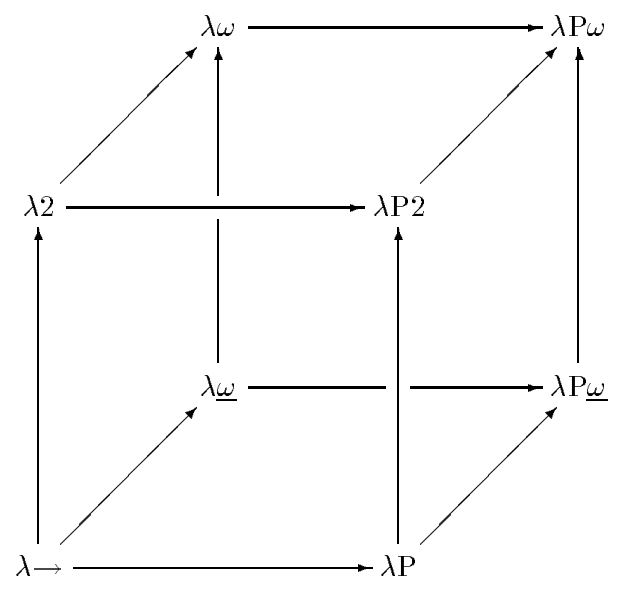
\includegraphics[width=.5\columnwidth]{./img/lambda-cube.png}%
	\end{center}
	\caption{Ламбда-куб Барендрегта, иллюстрирующий многообразие систем типизации с точки зрения четырех базовых видов зависимостей между типами и объектами: термов от термов, термов от типов, типов от типов и типов от термов.}%
	\label{pic:lambda-cube-long-caption}%
\end{figure}

\subsection{Ссылки на литературу}

В этой версии шаблона используется BibLaTeX, основанный на biber и BibTeX.
Поэтому для оформления списка литературы используются два файла:
\texttt{thesis-bibl.tex} и \texttt{biblio.bib}. Использование BibTex дает ряд
преимуществ. Не нужно заботиться о порядке сортировки, это делается
автоматически; не нужно заботиться, на какие элементы библиографии есть ссылки
--- печатаются только использованные в тексте элементы. Кроме того, многие
курсовые проекты выполняются на протяжении ряда лет. С BibTex проще собирать
список литературы и управлять им.

Ссылки на литературу даются посредством команды \texttt{\textbackslash{}cite},
например~\cite{Lermontov}, или~\cite{Pokrovski}. Ссылка является частью
предложения, поэтому должна идти до точки. Поддерживаются ссылки на несколько
источников сразу, к примеру~\cite{Borozda,Lagkueva,Methodology,Lermontov}.

На все элементы списка литературы должны быть ссылки из текста. При
использовании команды \texttt{\textbackslash{}cite} это происходит
автоматически. Отсутствиессылок на литературу из текста допускается в РСПЗ,
т.~е. в РСПЗ список литературы скорее имеет смысл списка подобранной литературы
по теме или библиографии. Для того, чтобы в списке литературы отобразились
источники, на которые отсутствуют ссылки в тексте, следует использовать команду
\texttt{\textbackslash{}nocite}. К примеру, \texttt{\textbackslash{}nocite\{*\}}
выводит в список литературы все содержимое подключенных BibTeX файлов, вставляя
невидимые ссылки на них.

\section{Сравнительный анализ алгоритмов \dots}

\dots





\section{Сравнительный анализ программных средств \dots}

\dots




\section{Выводы}

Тут пишем выводы по результатам анализа: что и с какой целью было проанализировано, какие выводы из этого сделаны, как они повлияли (должны повлиять) на дальнейший ход работы. Результаты анализа приводятся попунктно, основные вывода из проделанного анализа. Например:

\begin{enumerate}
	\item Выполнен сравнительный анализ таких-то формальных систем с точки зрения применимости к решению такой-то задачи. Ни одна из проанализированных напрямую не подходит, поэтому требуется разработать вариацию на основе системы такой-то.
	\item Были проанализированы варианты программных архитектур на основе систем. С учетом требований к поддержке больших объемов данных и высоких требований к потенциалу модернизируемости, была выбрана за основу такая-то архитектура.
	\item Сравнительный анализ таких-то библиотек показал, что библиотека X проще в использовании, но менее производительна, в то время как библиотека Y обеспечивает высокую производительность, но и требует значительных трудозатрат для использования. В связи с такими-то соображениями были принято решение использовать такую-то библиотеку.
\end{enumerate}



\section{Постановка задачи дипломной работы/курсового проекта}

Это всегда последний пункт. Далее пишется постановка задачи, на основе выданного задания. Это должен быть связный текст в объеме до 1-1,5 страниц. В этом разделе необходимо раскрыть цели и задачи УИРа/диплома. 

%%% Local Variables:
%%% TeX-engine: xetex
%%% eval: (setq-local TeX-master (concat "../" (seq-find (-cut string-match ".*-3-pz\.tex$" <>) (directory-files ".."))))
%%% End:
